\documentclass[border=3pt]{standalone}
% Preâmbulo compartilhado pelos diagramas TikZ da aula 4 de Navegação (Representação de Mapas)
\usepackage[T1]{fontenc}
\usepackage[utf8]{inputenc}
\usepackage{lmodern}
\usepackage{amsmath}
\usepackage{xcolor}
\usepackage{tikz}
\usetikzlibrary{arrows.meta,angles,quotes,decorations.pathmorphing,decorations.pathreplacing,calc,
                positioning,shapes.geometric,shapes.misc,backgrounds,fit,
                math}

% Paleta (mesma dos SVGs originais)
\definecolor{dblue}{HTML}{2A5B8C}
\definecolor{dorange}{HTML}{B3541E}
\definecolor{dgreen}{HTML}{4A7C59}
\definecolor{dred}{HTML}{9C4B4B}
\definecolor{dcream}{HTML}{F4F1EA}
\definecolor{dshade}{HTML}{DDD7C9}

% Função gaussiana (não normalizada por padrão de escala visual)
\pgfmathdeclarefunction{gauss}{3}{%
  \pgfmathparse{1/(#3*sqrt(2*pi))*exp(-((#1-#2)^2)/(2*#3^2))}%
}

% Estilos comuns (prefixo d... para não colidir com chaves internas do pgf)
\tikzset{
  >={Stealth[length=2mm]},
  dguide/.style={gray!55, dashed, line width=0.4pt},
  daxis/.style={gray!60, line width=0.7pt, ->},
  dbody/.style={fill=black!3, draw=black!80, line width=1pt},
  dacc/.style={draw=dblue, line width=1pt},
  dlbl/.style={black!55, font=\small},
  dsub/.style={black!45, font=\footnotesize},
  dstate/.style={circle, draw=black!80, fill=dcream, line width=1pt,
                 minimum size=17mm, font=\large, inner sep=1pt},
  dobs/.style={circle, draw=black!80, fill=dshade, line width=1pt,
               minimum size=14mm, font=\large, inner sep=1pt},
  dbox/.style={rounded corners=2pt, draw=black!80, fill=dcream, line width=1pt,
               align=center, inner sep=6pt},
  dop/.style={circle, draw=black!80, fill=white, line width=1pt,
              minimum size=6mm, inner sep=0pt, font=\small},
  dtrans/.style={->, dblue, line width=1pt},
  dmeas/.style={->, dorange, line width=1pt},
  dcurve/.style={line width=1pt, dblue},
  dcurveb/.style={line width=1.4pt, dorange},
}

\begin{document}
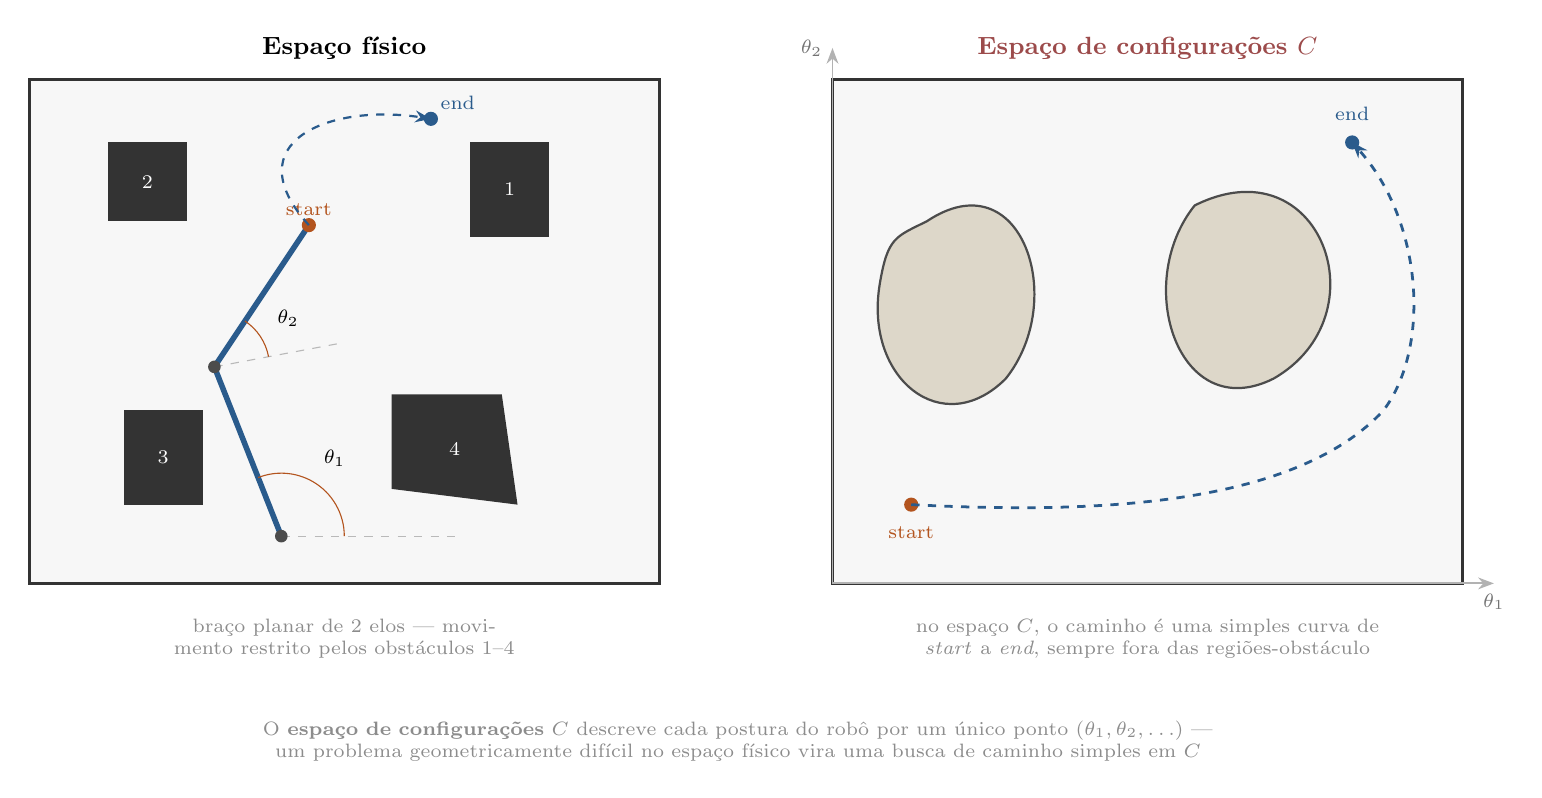
\begin{tikzpicture}[x=1cm,y=1cm]

  % Painel A: espaço físico com braço de 2 elos
  \begin{scope}[shift={(0,0)}]
    \draw[dbody, line width=1.2pt] (0,0) rectangle (8,6.4);
    \node[font=\bfseries\small] at (4,6.8) {Espaço físico};

    \fill[black!80] (5.6,4.4) rectangle (6.6,5.6);
    \node[dlbl, font=\scriptsize] at (6.1,5.0) {\textcolor{white}{1}};
    \fill[black!80] (1.0,4.6) rectangle (2.0,5.6);
    \node[dlbl, font=\scriptsize] at (1.5,5.1) {\textcolor{white}{2}};
    \fill[black!80] (1.2,1.0) rectangle (2.2,2.2);
    \node[dlbl, font=\scriptsize] at (1.7,1.6) {\textcolor{white}{3}};
    \fill[black!80] (4.6,1.2) -- (6.2,1.0) -- (6.0,2.4) -- (4.6,2.4) -- cycle;
    \node[dlbl, font=\scriptsize] at (5.4,1.7) {\textcolor{white}{4}};

    \coordinate (base) at (3.2,0.6);
    \coordinate (elbow) at (2.35,2.75);
    \coordinate (tip) at (3.55,4.55);
    \coordinate (baseguide) at (5.4,0.6);
    \coordinate (elbowguide) at (3.95,3.05);

    \draw[dguide] (base) -- (baseguide);
    \draw[dguide] (elbow) -- (elbowguide);
    \draw[dacc, line width=2pt] (base) -- (elbow) -- (tip);
    \fill[black!70] (base) circle (0.08);
    \fill[black!70] (elbow) circle (0.08);
    \fill[dorange] (tip) circle (0.09);

    \pic[draw=dorange, angle radius=8mm, angle eccentricity=1.5, "{\scriptsize $\theta_1$}"] {angle=baseguide--base--elbow};
    \pic[draw=dorange, angle radius=7mm, angle eccentricity=1.6, "{\scriptsize $\theta_2$}"] {angle=elbowguide--elbow--tip};

    \node[dorange, font=\scriptsize, anchor=south] at (tip) {start};
    \fill[dblue] (5.1,5.9) circle (0.09);
    \node[dblue, font=\scriptsize, anchor=south west] at (5.1,5.9) {end};
    \draw[dblue, dashed, line width=0.8pt, ->] (tip) .. controls (2.6,5.6) and (3.8,6.1) .. (5.1,5.9);

    \node[dsub, font=\scriptsize, align=center, text width=7.5cm] at (4,-0.7)
       {braço planar de 2 elos --- movimento restrito pelos obstáculos 1--4};
  \end{scope}

  % Painel B: espaço de configurações
  \begin{scope}[shift={(10.2,0)}]
    \draw[dbody, line width=1.2pt] (0,0) rectangle (8,6.4);
    \node[font=\bfseries\small, dred] at (4,6.8) {Espaço de configurações $C$};
    \draw[daxis] (0,0) -- (8.4,0) node[below, dlbl, font=\scriptsize] {$\theta_1$};
    \draw[daxis] (0,0) -- (0,6.8) node[left, dlbl, font=\scriptsize] {$\theta_2$};

    \fill[dshade, draw=black!70, line width=0.8pt]
      (1.2,4.6) .. controls (2.4,5.4) and (3.0,3.6) .. (2.2,2.6)
      .. controls (1.4,1.8) and (0.4,2.6) .. (0.6,3.8)
      .. controls (0.7,4.4) and (0.8,4.4) .. (1.2,4.6) -- cycle;
    \fill[dshade, draw=black!70, line width=0.8pt]
      (4.6,4.8) .. controls (6.2,5.6) and (7.0,3.4) .. (5.6,2.6)
      .. controls (4.4,2.0) and (3.8,3.8) .. (4.6,4.8) -- cycle;

    \fill[dorange] (1.0,1.0) circle (0.09);
    \node[dorange, font=\scriptsize, anchor=north] at (1.0,0.85) {start};
    \fill[dblue] (6.6,5.6) circle (0.09);
    \node[dblue, font=\scriptsize, anchor=south] at (6.6,5.75) {end};

    \draw[dblue, dashed, line width=1pt, ->] (1.0,1.0) .. controls (3.0,0.9) and (5.8,0.9) .. (7.0,2.2)
       .. controls (7.6,3.0) and (7.5,4.6) .. (6.6,5.6);

    \node[dsub, font=\scriptsize, align=center, text width=7.5cm] at (4,-0.7)
       {no espaço $C$, o caminho é uma simples curva de \textit{start} a \textit{end}, sempre fora das regiões-obstáculo};
  \end{scope}

  \node[dsub, font=\scriptsize, align=center, text width=17.5cm] at (9,-2.0)
     {O \textbf{espaço de configurações} $C$ descreve cada postura do robô por um único ponto $(\theta_1,\theta_2,\ldots)$ --- um problema geometricamente difícil no espaço físico vira uma busca de caminho simples em $C$};

\end{tikzpicture}
\end{document}
